%%%%%%%%%%%%%%%%%%%%%%%%%%%%%%%%%%%%%%START PREAMBLE 
\documentclass{article}
\usepackage{Sweave}
\usepackage{graphicx}
\usepackage{tabularx}
\usepackage{hyperref}
\usepackage{natbib}
\usepackage{pdflscape}
\usepackage{array}
\usepackage{authblk}
\usepackage{gensymb}

\usepackage[small]{caption}

\setkeys{Gin}{width=0.8\textwidth} %make the figs 50 perc textwidth
\setlength{\captionmargin}{30pt}
\setlength{\abovecaptionskip}{10pt}
\setlength{\belowcaptionskip}{10pt}
\topmargin -1.5cm    
\oddsidemargin -0.04cm  
\evensidemargin -0.04cm % same as oddsidemargin but for left-hand pages
\textwidth 16.59cm
\textheight 21.94cm 
%\pagestyle{empty}    % Uncomment if don't want page numbers
\parskip 7.2pt      % sets spacing between paragraphs
\parindent 0pt% sets leading space for paragraphs
\usepackage{setspace}
\renewcommand{\baselinestretch}{1.8}
\usepackage{lineno}
%%%%%%%%%%%%%%%%%%%%%%%%%%%%%%%%%%%%%%END PREAMBLE THAT IS THE SAME FOR ALL EXAMPLES

%Start of the document
\begin{document}

%\SweaveOpts{concordance=FALSE}
\Sconcordance{concordance:photoperiod.tex:photoperiod.Rnw:%
1 249 1}


\bibliographystyle{..//..//refs/bibstyles/ecology.bst}
\title{Spatial and temporal shifts in photoperiod with climate change} % perspective paper for OSPREE analyses


\author[1,2,a]{A. K. Ettinger (ailene.ettinger@tnc.org, ORCID ID:  0000-0002-6228-6732, twitter: @AileneKane)}
\author[2,3]{D. M. Buonaiuto (dbuonaiuto@g.harvard.edu, ORCID ID: 0000-0003-4022-2591)}

\author[2,3]{C. J. Chamberlain (cchamberlain@g.harvard.edu, ORCID ID: 0000-0001-5495-3219)}

\author[2,3,4,5]{I. Morales-Castilla (ignacio.moralesc@uah.es, ORCID ID: 0000-0002-8570-9312, twitter: @GloCEE\_EcoEvo)}

\author[2,3,6]{E. M. Wolkovich (e.wolkovich@ubc.ca, ORCID ID: 0000-0001-7653-893X)}

\affil[1]{The Nature Conservancy, Seattle, Washington, USA 98121}

\affil[2]{Arnold Arboretum of Harvard University, Boston, Massachusetts, USA 02130}


\affil[3]{Department of Organismic and Evolutionary Biology, Harvard University, Cambridge, Massachusetts, USA 02138}

\affil[4]{Department of Life Sciences, University of Alcal\`a CTRA N-II, KM., 33,600, 28802, Alcal\`a de Henares, Spain}

\affil[5]{Department of Environmental Science and Policy, George Mason University, Fairfax, Virginia, USA 22030}
 
\affil[6]{Forest \& Conservation Sciences, Faculty of Forestry, University of British Columbia, Vancouver, British Columbia, Canada V6T 1Z4}

\affil[a]{Corresponding author; phone: 781-296-4821; mailing address: 74 Wall Street, Seattle, WA 98121 USA}

\date{Article acceptance date: December 8, 2020} 

\maketitle %put the fancy title on
\textbf{Statement of authorship} 
All authors conceived of this manuscript and each contributed data analysis and figures. AKE wrote the manuscript, and all authors contributed revisions to the manuscript. 

\textbf{Data Accessibility} The OSPREE database is publicly archived at KNB, doi:10.5063/F1CZ35KB. \citep{wolkovich2019}.

\textbf{Running head} Shifts in photoperiod with climate change

\textbf{Key words} phenology, global warming, range shifts, timing, spring, budburst,daylength 

\textbf{Paper type} `Research review' or `Viewpoint'


%%%%%%%%%%%%%%%%%%%%%%%%%%%%%%%%%%%%%%%%%%%%%%%%%%%

%%%%%%%%%%%%%%%%%%%%%%%%%%%%%%%%%%%%%%%%%%%%%%%%%%%
\newpage
\linenumbers
\section*{Abstract}
Climate change causes both temporal (e.g., advancing spring phenology) and geographic (e.g., range expansion poleward) species shifts, which affect the photoperiod experienced at critical developmental stages (`experienced photoperiod'). As photoperiod is a common trigger of seasonal biological responses---affecting woody plant spring phenology in 87\% of reviewed studies that manipulated photoperiod---shifts in experienced photoperiod may have important implications for future plant distributions and fitness. However, photoperiod has not been a focus of climate change forecasting to date, especially for early-season (`spring') events, often assumed to be driven by temperature. Synthesizing published studies, we find that impacts on experienced photoperiod from temporal shifts could be orders of magnitude larger than from spatial shifts (1.6 hours of change for expected temporal versus one minute for latitudinal shifts). Incorporating these effects into forecasts is possible by leveraging existing experimental data; we show that results from growth chamber experiments on woody plants often have data relevant for climate change impacts, and suggest that shifts in experienced photoperiod may increasingly constrain responses to additional warming. Further, combining modeling approaches and empirical work on when, where, and how much photoperiod affects phenology could rapidly advance our understanding and predictions of future spatio-temporal shifts from climate change. 

\newpage
\section*{Introduction}

\par Shifts in phenology---i.e., the timing of biological events, including budburst, leafout, and flowering in plants, as well as bird arrival, egg hatching and myriad other biological activities---are some of the most widely documented signals of climate change. Spring phenology in particular has shifted, occurring earlier as temperatures warm, with average shifts of 1.2 to 5.1 days earlier per decade \citep{bradley1999,parmesan2003, poloczanska2013,root2003} or 1.3 to 5.6 days earlier per \degree C of warming \citep{polgar2013,Wolkovich:2012n}. These changes are some of the largest climate change-induced shifts observed, with early spring phenology shifting more rapidly than later season phenology in most cases \citep{bradley1999,menzel2006}. 

\par Phenology is not controlled solely by temperature, however. Photoperiod is also a critical cue, signaling changes in growth and reproduction across diverse species \citep[e.g.,][]{flynn2018,lagercrantz2009,bradshaw2007,Howe:1996,solbakken1994}. Even spring phenology, which is highly temperature-sensitive, is thought to be determined interactively by photoperiod and temperature \citep[][see also Box 1]{fu2019}. Photoperiod is a useful cue to synchronize activities with seasonal climatic changes \citep[e.g.,][]{Singh:2017, Basler:2012, Hsu:2011} because it is consistent across years, especially compared to other cues such as temperature and precipitation \citep{saikkonen2012}.  For example, relying on a threshold photoperiod (see Table 1), rather than temperature alone, may prevent woody plants from leafing out during `false spring' events \citep[unusually warm periods during winter and early spring that are followed by a return to cold temperatures,][]{gu2008}. 

\par Recent studies suggest that photoperiod cues may eventually restrict phenology in a warmer world. With additional climate change, photoperiod may limit phenological shifts of certain species such that they will not track rising temperatures \citep{fu2015,way2015,Basler:2012,koerner2010a}. The idea of photoperiod constraints is controversial, however, as other studies suggest that photoperiod will not slow responses to warming for most species \citep{chuine2010,zohner2016}. Resolving this debate requires a greater understanding of the extent to which daylength constrains phenology and how rapidly photoperiod responses can acclimate or adapt to new environmental conditions \citep{grevstad2015}.

\par Perhaps because of these variable and uncertain responses, photoperiod is often not included in forecasts of biological responses to climate change, especially in the spring, even though it is known to be an important cue for biological activity \citep[but see ][]{duputie2015,grevstad2015,Caffarra:2011qf}. The exclusion of photoperiod may be problematic: although photoperiod itself is stable over time, the photoperiod that species \emph{experience} at critical developmental stages (henceforth, `experienced photoperiod'), as they undergo climate change-induced shifts in space and time, is likely to be much less stable (Fig. \ref{fig:spacetime}). This shift in experienced photoperiod extends to distributional shifts due to climate change, as many species' distributions have moved poleward and upward in elevation \citep[i.e., range shifts,][]{chen2011,harsch2009,parmesan2006,penuelas2003}. 
\par The implications of potential climate change-induced shifts in experienced photoperiod are unclear, as the magnitudes of potential shifts have not been described. Effects of photoperiod shifts may be relatively minor, especially compared to the substantial year-to-year variation in experienced photoperiod (Fig. \ref{fig:greenup}). Alternatively, photoperiod may begin to constrain species' responses to climate change \citep{huffeldt2020,fu2015,way2015,Basler:2012,koerner2010a}.

\par Here, we ask: 
\begin{enumerate}
\item How will climate change alter experienced photoperiod for plants? 
\item What are the implications of altered experienced photoperiods for plant responses to climate change?
\item Can researchers apply data from experiments that alter photoperiod to improve forecasts of biological implications of climate change?

\end{enumerate}
\par Our questions are broadly relevant for diverse species and seasonal events. We use a case study of spring woody plant phenology to illustrate several of our points (Boxes 1 \& 2). We focus on spring events, as phenology during this time is one of the most widely observed and rapidly changing biological responses to climate change \citep{parmesan2006}. In addition, the role of photoperiod is less understood in spring phenology compared with autumn phenophases \citep[reviewed in, e.g.,][]{azeez2015,gallinat2015,gill2015,lagercrantz2009, allona2008}, but recent studies showing declines in responses of spring budburst to warming \citep[e.g.,][]{fu2019,gusewell2017,yu2010} suggest that photoperiod constraints may be imminent. 

\section*{How will climate change alter experienced photoperiod for plants?}
\par Species experience different photoperiod regimes depending on their location on Earth, the seasonal timing of their activity, and inter-annual variation in climate (Fig. \ref{fig:spacetime}). Consider, as an example, the daylength experienced by plants on the date that spring `green-up' occurs. We use green-up date as an example because it represents an important spring event, signaling the start of the growing season, and global estimates are available. Photoperiod on green-up date varies with latitude (Fig. \ref{fig:greenup}A), in part because latitudinal variation in green-up date, which occurs earlier toward the equator and later toward the poles, is strongly driven by climatic differences that affect phenology, and in part because of latitudinal variation in photoperiod (e.g., at the poles, the daylength at the summer solstice is 24 hours; see also Fig. \ref{fig:spacetime}). (See ``Quantifying and mapping differences in green-up across the United States and Europe'' in the \emph{Methods S1} for additional details of this analysis.) 
\par Some consistent patterns in experienced photoperiod are apparent at a broad scale. Across years, photoperiod at green-up is longer toward the poles (i.e., on the day of year when green-up occurs close to the north pole, daylength approaches 24 hours in both an average year, Fig. \ref{fig:greenup}A, and in an early year, Fig. \ref{fig:greenup}B). In addition, green-up does not appear to occur at daylengths less than 10 hours across North America and Europe. 
\par Despite these consistent broad-scale patterns, there is also strong spatiotemporal variation in experienced photoperiod across years. Comparing the photoperiod at green-up in an `early' versus an `average' year (Fig. \ref{fig:greenup}A,B) shows that experienced photoperiod at green-up can vary by two to three hours from one year to the next in the same location (Fig. \ref{fig:greenup}C).

\par Against this existing background variation, climate change will cause shifts in experienced photoperiod as species respond to warming temperatures. Spatial shifts in species' ranges and temporal shifts in phenology will alter the photoperiods experienced by organisms with future climate change. The magnitude of these alterations will vary depending on the organism's location and the type of shift(s) it undergoes. For example, poleward shifts in species' ranges cause plants to experience a wider range of daylength throughout the year (Fig. \ref{fig:spacetime}), which may pose challenges to organisms undergoing temperature-induced poleward range shifts \citep{huffeldt2020}. Elevational shifts, in contrast, cause minimal change to the range of daylength throughout the year.

\par To date, most focus on shifts in photoperiod with climate change has centered on how spatial range shifts will affect photoperiod \citep[e.g.,][]{huffeldt2020,way2015,saikkonen2012}. However, shifting phenology---especially the large changes seen in spring phenology---will also alter experienced photoperiod, because of the seasonal patterns of daylength (Fig. \ref{fig:spacetime}). 

\par Current data suggest that temporal shifts will yield much larger changes in experienced photoperiod than latitudinal shifts (Fig. \ref{fig:spacetime}).
Consider a tree species that bursts its buds at latitude 45$^{\circ}$, on average around day of year 91 (April 2), when daylength is 12.8 hours. If the species' phenology shifts 30 days earlier over the next century \citep[i.e., a rate of ~3 days per decade, as has been observed,][]{parmesan2003}, it will experience a daylength that is 1.6 hours shorter. This 1.6 hour decrease in daylength is equivalent to moving up 28.5$^{\circ}$ in latitude on this day of year. However, if the same species shifts its range up in latitude 0.5$^{\circ}$ \citep[i.e., 60 km over the next century, comparable to observed rates,][]{chen2011,parmesan2003}, it will experience a daylength that differs by less than a minute on the same day of year. 
\par Temporal shifts in temperate areas are likely to yield larger changes in experienced photoperiod for autumn phenology, as well. Consider again the tree at latitude 45$^{\circ}$, which may senescence on day of year 300 (October 27), on average \citep{gill2015}, when daylength is 10.5 hours. If senescence shifts 33 days later over the next century \citep[i.e., a rate of 3.3 days per decade, as has been observed,][]{gill2015}, it will experience, at the end of the growing season, a daylength that is 1.3 hours shorter. This is equivalent to moving up 16$^{\circ}$ in latitude on this day of year.
\section*{What are the implications of altered photoperiods for plant responses to climate change?}
Climate change alters the experienced photoperiod, but the implications of this change for plants are currently unclear, in part, because phenology both affects and is affected by experienced photoperiod: climate change-induced shifts in phenology alter experienced photoperiod, which in turn affects phenology. Daylength, often in combination with temperature, can play a role in controlling critical biological functions, including vegetative growth, cell elongation, budburst, and flowering in plants \citep{fu2019,Heide:2012aa,Heide:2011aa,Hsu:2011,sidaway2010,mimura2007,Linkosalo:2006aa,erwin1998,Ashby:1962aa}.
Climate change-induced shifts in photoperiod are therefore likely to alter these functions. 

\par Growth chamber studies show that the magnitude of daylength shifts expected with climate change (i.e., 1-2 hours of difference in daylength with temporal shifts over the next century) are substantial enough to affect spring phenology in trees (Table S1). The direction and magnitude of responses will vary, however, because of variation in photoperiod sensitivity, and because photoperiod often interacts with other environmental drivers, such as temperature, to affect phenology (Box 1). 

\par The climate change-induced trend toward ever-earlier springs means that experienced photoperiod may increasingly approach threshold photoperiods (see Table 1) for many species, potentially constraining their ability to respond to additional warming \citep{fu2019,vitasse2013,koerner2010a,Morin:2010aa,Nienstaedt:1966aa}. Interactions between photoperiod and temperature may therefore result in muted phenological shifts, compared to what would be expected based on temperature change alone \citep{koerner2010a,mimura2007,wareing1956}. This has been a topic of much interest in the climate change literature because it predicts that as photoperiod becomes limiting, average trends of earlier spring phenology \citep{polgar2013,penuelas2002,menzel2000} and later autumn senescence \citep{gill2015,richardson2018} with warming may stop. 
 \par A challenge in predicting if or when the trends of shifting phenology with warming may slow or stop abruptly is the wide range of observed photoperiod sensitivity (see Table 1) across events \citep[e.g., spring versus fall events][]{mimura2010}, species \citep{flynn2018,zohner2016,Sanz-Perez:2009aa}, latitudes \citep{ettinger2020,Partanen:2005aa,johnsen1996}, populations \citep{gauzere2017,saikkonen2012,Caffarra:2011b,bradshaw2007,Vihera-Aarnio:2006aa}, and ecotypes \citep{Howe:1995aa}. How much genotype versus environment explain this variation is an active area of research \citep[e.g.,][]{frejaville2019,franks2014,gould2010,mimura2010}. Environmental conditions clearly play a role: different combinations of ambient temperature and photoperiod may explain some of this variation, and temperature cues can override photoperiod requirements under certain conditions \citep [e.g.,][] {tanino2010}. In such cases, future climate change-induced phenological shifts may occur at different rates than past shifts with warming. On the other hand, some of this variation may be due to underlying genetic differences driven by local adaptation, because photoperiod responses can be under strong genetic control \citep[][see also Boxes 1, 2]{keller2011,weih2004,bradshaw1995}. Differences in genetic control of photoperiod may be pronounced across spring versus fall events, as research suggests stronger local adaptation in photoperiod cues for budset than budburst \citep{mimura2010}, though to date much research focuses on spring or fall events separately, making a robust comparison difficult. Valuable advances to the field may be achieved by increased efforts to compare controls on phenological events across the growing season and how they may be connected, through carbon dynamics or other factors \citep{zani2020,ettinger2018}. Further teasing out the relative roles of genetics versus environmental conditions on phenology will be critical to accurate forecasts under climate change \citep{pau2011}.

\par Species- and population-level variation in photoperiod sensitivity may scale up to alter communities as climate change progresses. For example, a species or population that is relatively insensitive to photoperiod can take advantage of warmer springs by having an earlier start to its growing season. Indeed, phenological tracking of temperature (e.g., earlier flowering, leafout or migration with warming) has been linked with higher performance in plants and animals \citep{cleland2012,muir1994,willis2010}. Species or populations that are sensitive to temperature but relatively insensitive to photoperiod may therefore outcompete slower-growing or later-emerging ones that are limited by photoperiod and thus cannot take advantage of longer growing season conditions. Not all studies, however, find links between performance and high sensitivity to temperature \citep[e.g.,][]{block2020}, and early-season species in most temperate zones risk losing tissue to frost \citep{frostbook}. Thus, the advantages of tracking warming may depend on how quickly mean temperatures versus last frost dates shift \citep[e.g.,][]{inouye2002}, such that in some systems photoperiod cues could prevent species from starting growth or reproduction too early (when they risk losing their investments in new tissue). To identify where, when, and how communities may be altered therefore requires quantifying species- and potentially population-specific temperature and photoperiod sensitivities, and developing methods that incorporate both photoperiod and environmental events that impact fitness (such as frosts).

\section*{Future directions: outstanding questions and incorporating photoperiod into forecasting}
\par The complexity of photoperiod effects on phenology and how warming alters experienced photoperiod highlights that future rates of phenological shifts are unlikely to be straightforward extrapolations from past and current rates. Statistical and process-based models---the two broad categories of forecasting approaches---both acknowledge this difficulty, but differ importantly in how they relate phenology to climate change. Statistical models relating phenology to climate change typically assume linear relationships between species' responses and environmental variables \citep[e.g., ][]{flynn2018,ibanez2010}, whereas process-based models often incorporate nonlinear threshold relationships \citep[e.g.][]{chuine2001,morin2009}. Further, statistical models of phenology under climate change often ignore photoperiod, focusing instead on seasonal or annual temperature \citep[e.g.][but see \citet{richardson2013}]{diez2012,ibanez2010}, whereas process-based models of phenology more frequently incorporate photoperiod, along with temperature \citep{lundell2020,duputie2015,zhao2013,morin2009}. Process-based models may thus seem superior for integrating photoperiod, but they can be challenging to develop, requiring detailed data that are often not readily available (e.g., daily climate data, nonlinear biological responses to fine-scale changes in temperature). Perhaps because of this, statistical models remain more commonly used in climate change forecasts of biological responses \citep[e.g.,][]{garcia2016,Basler:2012,diez2012,zhu2012,ibanez2010}.

\par Future modelling of spring plant phenology can incorporate photoperiod by leveraging the large amount of experimental data on photoperiod responses (e.g., for woody plants, see Fig. \ref{fig:photomap}, Table S1, Box 1), especially when process-based approaches are used. Researchers can use these data to first learn whether the study species (or a phylogenetically closely related species) shows a photoperiod effect and, ideally, identify its threshold photoperiod and how it varies by population, ecotype, or other factors \citep{tobin2008,bradshaw2006}. If there is evidence of a photoperiod response (e.g., \emph{Fagus grandifolia}, or \emph{Tilia americana} with low chilling, shown in Fig. \ref{fig:photocurve}), daylength should be added to forecasting models. We suggest initial models could use a threshold photoperiod to define short-day and long-day conditions (Fig. \ref{fig:condiag}, Box 1), then test how much the addition alters forecasts. Given the large change in experienced photoperiod with temporal shifts (Fig. \ref{fig:spacetime}), this may be particularly important for phenological forecasting. Since spatial shifts are associated with smaller changes in experienced photoperiod, it may be less important for distribution forecasts. Many species, however, may shift in \emph{both} space and time simultaneously. Thus, even though experienced photoperiod changes little as species distributions shift in space, phenology may be altered significantly if the newly expanded portions of the range contain novel environmental conditions \citep[e.g., ][]{martin2014}.

\par For some species, experimental data can be immediately used in forecasting because experiments manipulate photoperiod at relevant scales \citep[e.g., ][Fig. \ref{fig:photomap}, Box 1, Table S1]{Heide:2015aa,Basler:2014aa}. For example, photoperiod treatments from growth chamber experiments with \emph{Fagus sylvatica} span the variation in both current and expected future ranges \citep[Box 1, ][]{duputie2015}, and may allow identification of threshold photoperiods (Fig. \ref{fig:condiag}). In other cases, attempting to incorporate photoperiod into forecasts of future phenology will reveal gaps in our understanding of many aspects of photoperiod responses. For example, photoperiod treatments from existing experiments of \emph{Quercus robur} do not accurately represent experienced photoperiods from current or future estimates (Box 1), making fine-scale projections difficult, even for this relatively well-studied species. This gap extends to many species, as most experiments manipulate photoperiod much more dramatically than will occur with climate change (Fig. \ref{fig:photomap}, Box 1). Although these studies can be useful for a mechanistic understanding of photoperiod responses, extrapolating them to climate change models may not be reasonable. 
 

\par Photoperiod is not fully integrated into most forecasts of biological responses to climate change \citep[but see][for an example in insects]{tobin2008}, an omission that could affect forecast accuracy. Photoperiod is incorporated into some ecosystem models \citep[e.g., the Ecosystem Demography model] []{jolly2005,medvigy2013} used for forecasting but not others \citep[e.g.,][]{richardson2012}, and is rarely included in species distribution models \citep[e.g.,][]{morin2009,zhu2012}. The sensitivity of model outcomes to assumptions made about experienced photoperiod and threshold responses to photoperiod needs further study, including understanding how variation in photoperiod responses across ecosystems, species, populations, and life stages impacts forecasts. 
We have focused here on spring phenology, but future work could also address the sensitivity of model outcomes to shifts in experienced photoperiod at the end of the growing season (e.g., leaf senescence and onset of dormancy). Autumn photoperiod affects photosynthesis, growth, and budset in woody plant species, and photoperiod-induced declines in photosynthetic capacity may constrain carbon sequestration even if warming prolongs leaf senescence \citep[][]{Howe:1996, bauerle2012,stinziano2017}.

\par As researchers more fully integrate experienced photoperiod into forecasting, a critical area of further study is understanding \emph{how} photoperiod acts as a cue. For some species, photoperiod responses are qualitiative (that is, there is a threshold photoperiod with long-day responses differing from short-day responses; see Table 1), whereas other species appear to exhibit quantitative responses to photoperiod \citep{wareing1956}. Photoperiod seems to interact with temperature to affect phenology \citep[e.g.,][]{zydlewski2014}; this would explain the divergent effects of photoperiod observed across studies in woody plants (Box 1). However, exactly how it interacts with temperature is not well-defined for most taxa. For many species, additional experimental and physiological research is necessary, since the dormancy-breaking processes that photoperiod affect require detailed physiological approaches to observe. Though the main ecophysiological processes involved in regulating phenology of woody plants are relatively well-documented, a  mechanistic understanding of the physiological, molecular, and genetic bases of dormancy is lacking \citep[Box 2,][]{hanninen2019, chuine2016}. In addition, photoperiod and temperature cues can differentially affect the phenology of distinct physiological processes in woody species, decoupling, for example, responses of growth or leaf development and carbon uptake to warming \citep{stinziano2017,bauerle2012}. Accounting for ecophysiological effects of photoperiod can result in quantifiable declines on modeled global gross primary production \citep{bauerle2012}, suggesting that including temporal and spatial shifts in experienced photoperiod with climate change may also alter global model estimates.
\par Understanding the drivers, as well as the consequences, of variation in photoperiod responses within and across individuals, populations, and species will be critical for forecasting.  Incorporating trait and/or phylogenetic frameworks may provide useful avenues for improving forecasts \citep{buckley2012}. For example, what traits are associated with photoperiod sensitivity and does variation in photoperiod sensitivity or related traits have a strong genetic component? If so, are species or populations from some locations or lineages more likely than others to be constrained by photoperiod in their responses to climate change? More accurate forecasts will facilitate improved understanding of the implications of shifts in experienced photoperiod for carbon sequestration under climate change at a global scale.

\section*{Conclusions}
Organisms may undergo large changes to the photoperiod they experience with climate change, even if they do not shift their ranges spatially. Here we have highlighted that these altered photoperiods may stall phenological shifts with future warming \cite[e.g., Table S1,][]{fu2019, gusewell2017,yu2010}, with cascading effects on growth, fitness, and community composition due to the large variation in photoperiod responses across species and populations (Box 1). We have focused on woody plant phenology, but shifts in photoperiod with climate change have implications for a variety of plant and animal responses, as daylength affects critical activities for species from insects \citep{bradshaw2006} and salmon \citep{taranger2003} to birds \citep{dawson2001} and marsupials \citep{mcallan2006}. Given what we know, incorporating photoperiod into forecasting of climate change responses should improve model accuracy (Fig. \ref{fig:condiag}), and will illuminate additional experiments that could improve our mechanistic understanding of photoperiod as a critical cue for diverse biological responses. 
\section* {Table 1. Glossary}
\begin{itemize}
\item \underline{budburst}: one or more leaf buds have visible green tips. 
\item \underline{chilling}: the intensity and duration of winter temperature, often a certain sum of chilling \citep[e.g., amount of hours or days of cold temperatures, defined by a specific critical temperature or range of temperatures, such as between 0 and 7.2 \degree C,][]{richardson1974} that is required to iniate budburst.
\item \underline{daylength}: the period of time during a 24-hour period during which an organism receives light.
\item \underline{dormancy}: halted or reduced growth or activity.
\item \underline{forcing}: warm spring temperatures, often a certain sum of forcing (e.g., amount of hours or days above a specific temperature) that is required before budburst can occur.
\item \underline{green-up}: the beginning of a new cycle of plant growth, usually evaluated at the landscape scale.
\item \underline{phenology}: the timing of life cycle events in organisms.
\item \underline{photoperiod}: the daily duration of light (daylength) and dark to which an organism is exposed; often used synonymously with daylength.
\item \underline{photoperiod sensitivity}: the degree to which phenology is controlled by daylength; may be a nonlinear, or `threshold', response in plants (Box 2).
\item \underline{photoperiodism}: the ability of an organism to assess or respond to length of day or night in its behavior, physiology, growth, development, or reproduction.
\item \underline{threshold photoperiod}: length of day that causes an organism to switch from a short-- to a long--day response (or vice verse). For example, in European larch (\emph{Larix decidua}), budburst development may be constrained under short-day conditions, when daylengths are less than a threshold photoperiod of 10-11 hours \citep{migliavacca2008}. Above this threshold photoperiod, the long-day response of unconstrained budburst development can occur.
\end{itemize}

\section*{Acknowledgements}
We thank the many researchers who conducted the experiments synthesized in this manuscript; H. Kharouba for helpful comments that improved the manuscript; B. Feist for improving the appearance of Fig. \ref{fig:photomap} dramatically; and A. Duputi\'e and I. Chuine for sharing projections from PhenoFit. The National Science Foundation (DBI 1401854 to AKE), NSERC Discovery Award (RGPIN-05038 to EMW), Canada Research Chair in Temporal Ecology (EMW), and Spanish Ministry for Science and Innovation (PID2019/109711RJ-100 to IM-C) provided funding. Any opinion, findings, and conclusions or recommendations expressed in this material are those of the authors and do not necessarily reflect the views of the National Science Foundation or The Nature Conservancy.
\bibliography{/Users/aileneettinger/Documents/GitHub/ospree/refs/ospreebibplus}
\clearpage

\section*{Supporting Information}:
\par Methods S1 includes additional details of the database and analyses performed.
\par Table S1 includes locations, photoperiod treatments, and whether or not photoperiod had an effect on budburst for studies in \citet{wolkovich2019} with atleast two photoperiod treatments. 

\section* {Figures}

\begin{figure}[h]
\centering
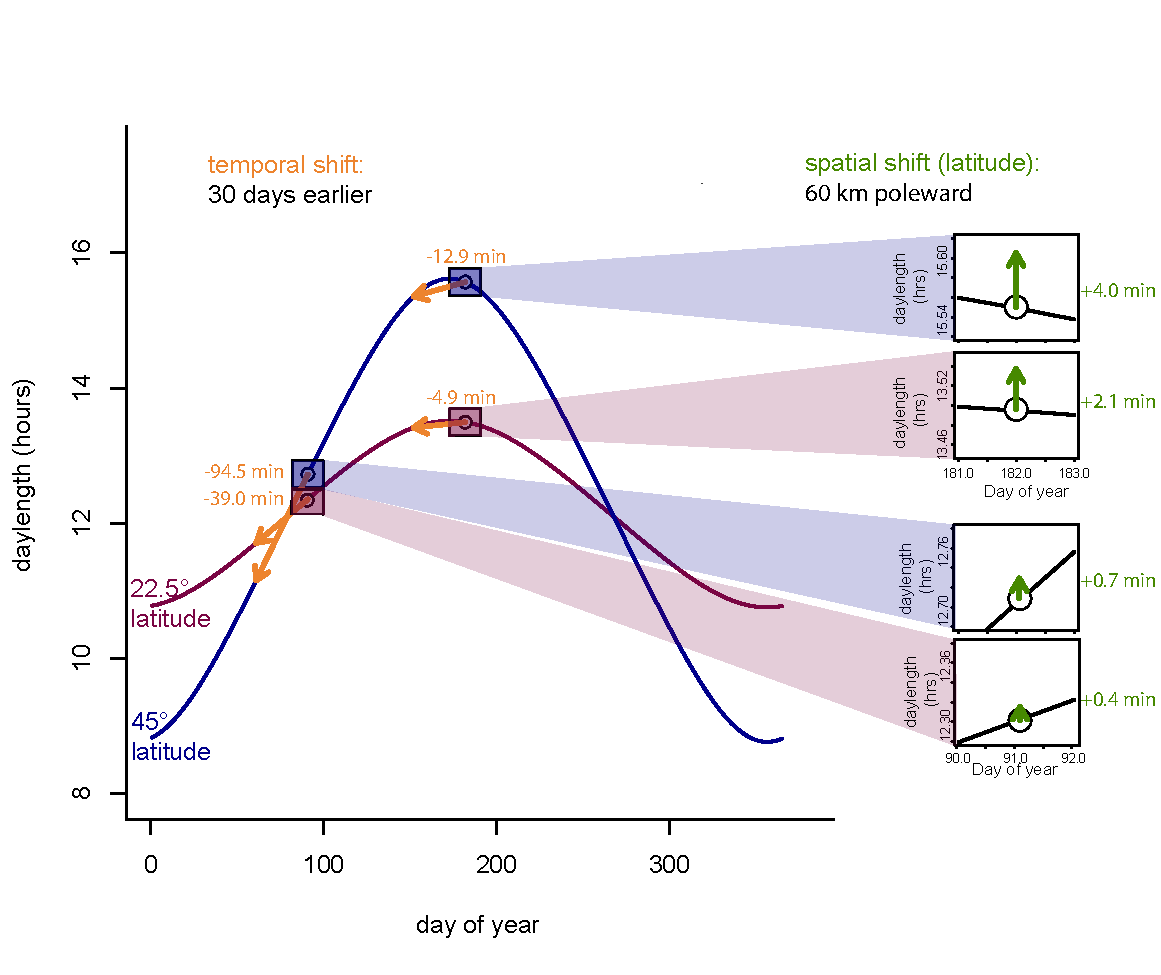
\includegraphics{..//..//analyses/photoperiod/figures/photo_spacetime_v4b_newcolors.pdf} %
\caption{\textbf{Temporal (i.e., phenological) shifts in activity yield larger changes in experienced photoperiod compared to spatial (i.e., latitudinal) shifts} on the same day of year, due to patterns in photoperiod variation with latitude and by day of year. Here, we show this variation at two latitudes (22.5$^{\circ}$, 45$^{\circ}$), using hypothetical spatial and temporal shifts. These shifts are based on observed rates with recent global warming: for spatial shifts, 6-17 kilometers per decade, or approximately 0.5-1.5$^{\circ}$ in 100 years \citep{parmesan2003,parmesan2006}; for temporal shifts, 3 days per decade, or 30 days in 100 years \citep{parmesan2006,chen2011}. These potential, plausible shifts highlight the greater magnitude in daylength changes from temporal shifts in the early spring, close to the vernal equinox (e.g., day of year 91), versus close to the summer solstice (e.g., day of year 182) at temperate latitudes.  It is also apparent that early spring temporal shifts at high latitudes result in more extreme changes in daylength than shifts at lower latitudes (e.g., a temporal shift 30 days earlier results in a reduction in daylength of 94.5 minutes at 45$^{\circ}$ versus 39.5 minutes at 22.5$^{\circ}$).}
 \label{fig:spacetime}%
 \end{figure}
 
 \begin{figure}[h]
\centering
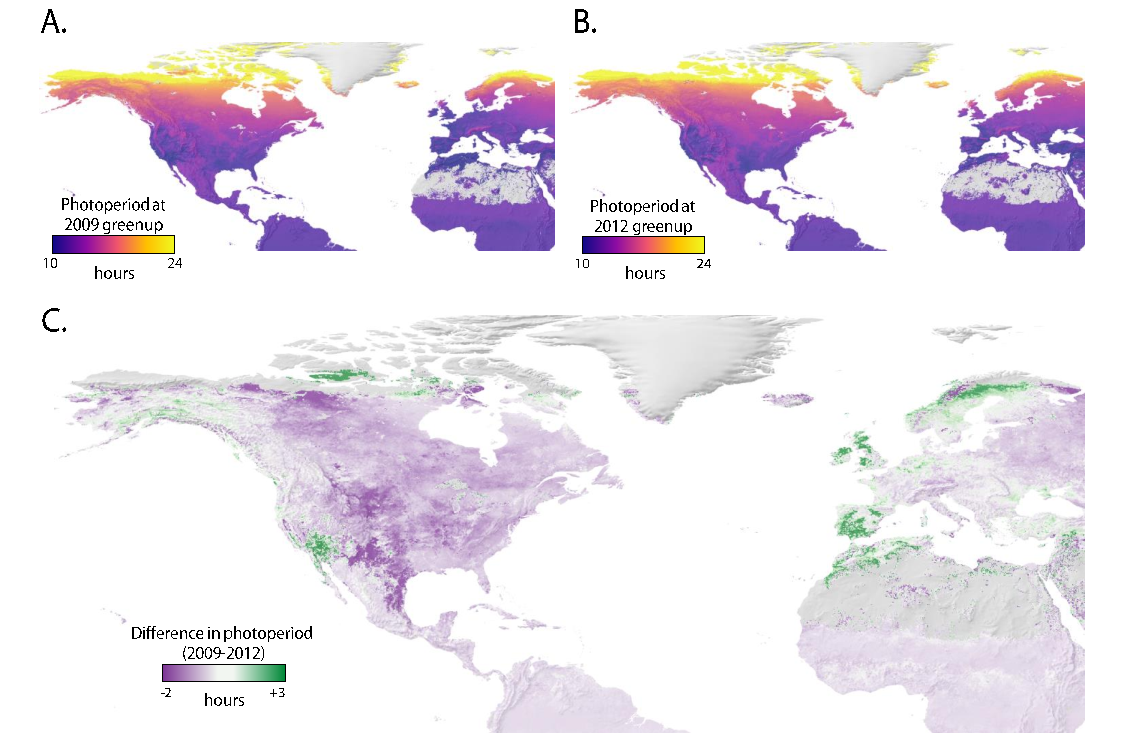
\includegraphics{..//..//docs/photoperiod/figures/Greenup_corr_sm_leg.pdf} %2009 greenup
\caption{\textbf{Photoperiod on `green-up' date varies over space and between years}. `Green-up' date is the beginning of seasonal greening, identified by satellite remote sensing measurements, taken regularly throughout the year, of concentrations of green leaf vegetation. Hours of daylight are shown on the date of spring green-up (here from MODIS satellite data) across North America and Europe for an average (2009, A) and early (2012, B) North American start of spring. The differences between the years (in hours of daylength) are shown in (C). A negative difference signifies earlier green-up in 2012 versus 2009; a positive difference is the result of later green-up in 2012 compared with 2009. See ``Quantifying and mapping differences in green-up across the United States and Europe'' in Methods S1 of the \emph{Supporting Information} for additional details. }%
 \label{fig:greenup}%
 \end{figure}

\begin{figure}[h]
\centering
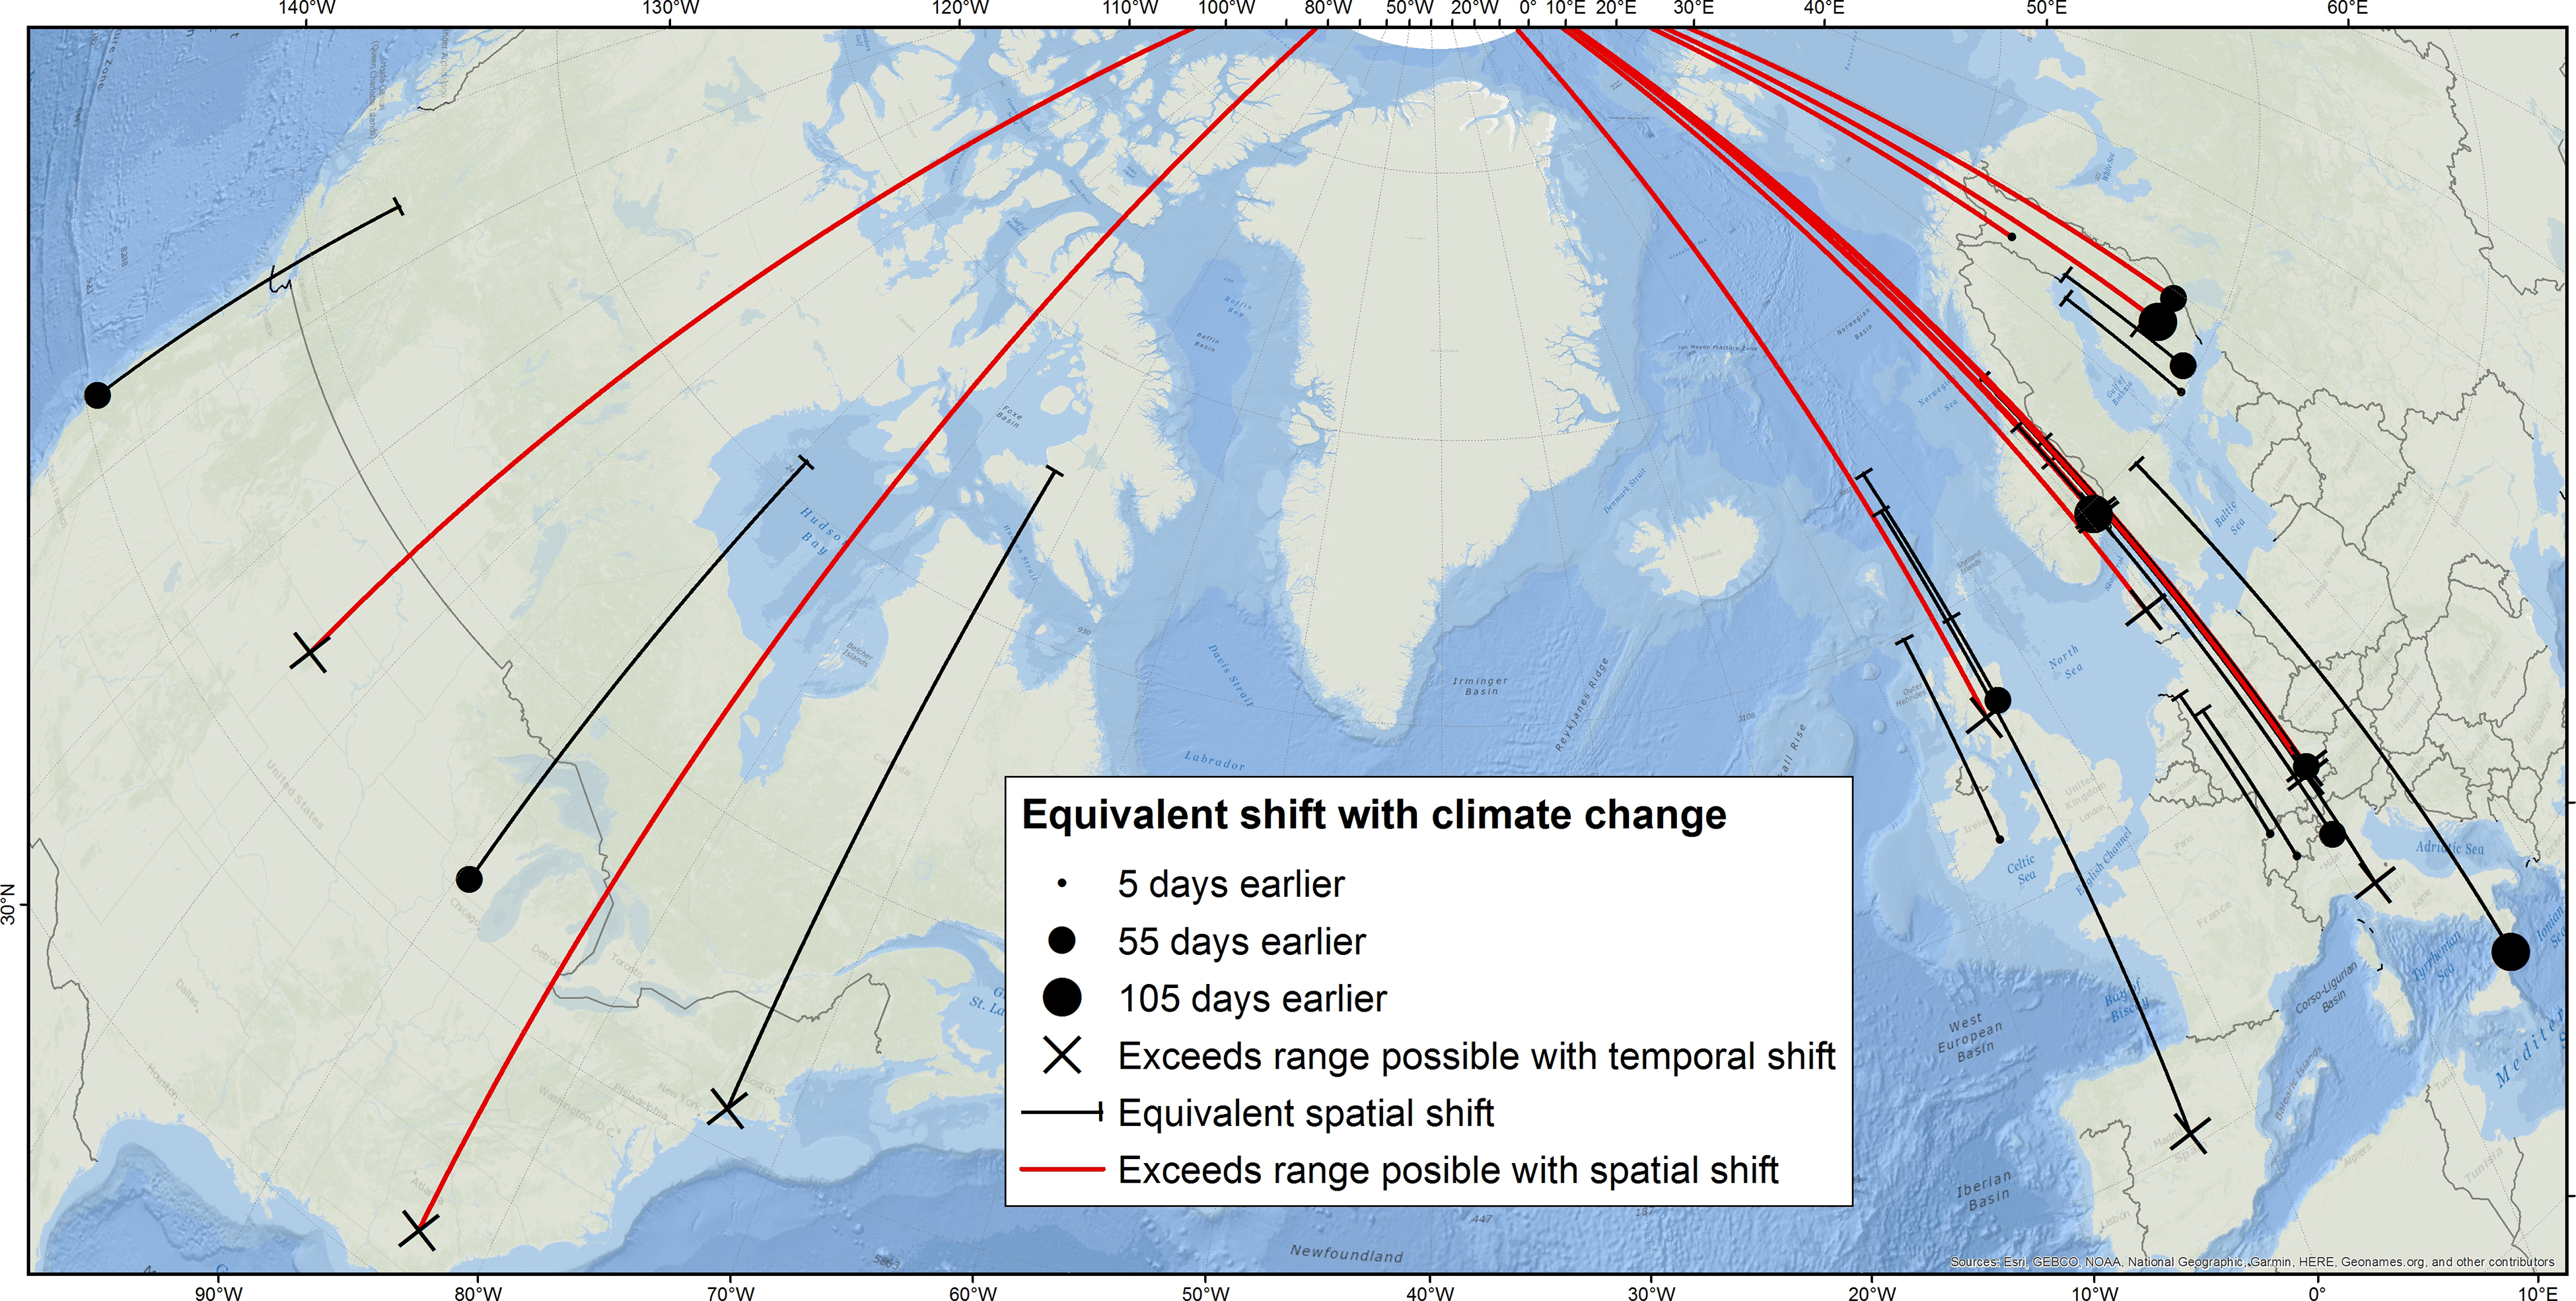
\includegraphics{..//..//analyses/photoperiod/figures/ospree_photopmap_fromblake.jpg} 
\caption{\textbf{A map of experimental photoperiod treatments from a meta-analysis of woody plant spring phenology and their equivalent spatial and temporal shifts} demonstrates that many experiments manipulate photoperiod more dramatically than will occur with climate change. Mapped points (circles and Xes) are locations of experiments in \citet{wolkovich2019} that manipulated photoperiod (30 total experiments; see Box 1). In 11 out of 30 cases, the difference between experimental treatments exceeded the range in photoperiod experienced across the entire year at the study latitude (Xs; circles mark temporal shifts within a possible range). Note that many studies occur at high latitudes, which experience a wide range of photoperiod across the year. In 13 out of 30 cases, the experimental treatment differences exceeded the photoperiod change that would be experienced with a latitudinal shift of up to 40$^{\circ}$ (red lines; black lines represent spatial shifts within a possible range). See ``Mapping temporal and spatial shifts in space and time'' in Methods S1 of the \emph{Supporting Information} for additional details. }
 \label{fig:photomap}
 \end{figure}


\begin{figure}[h]
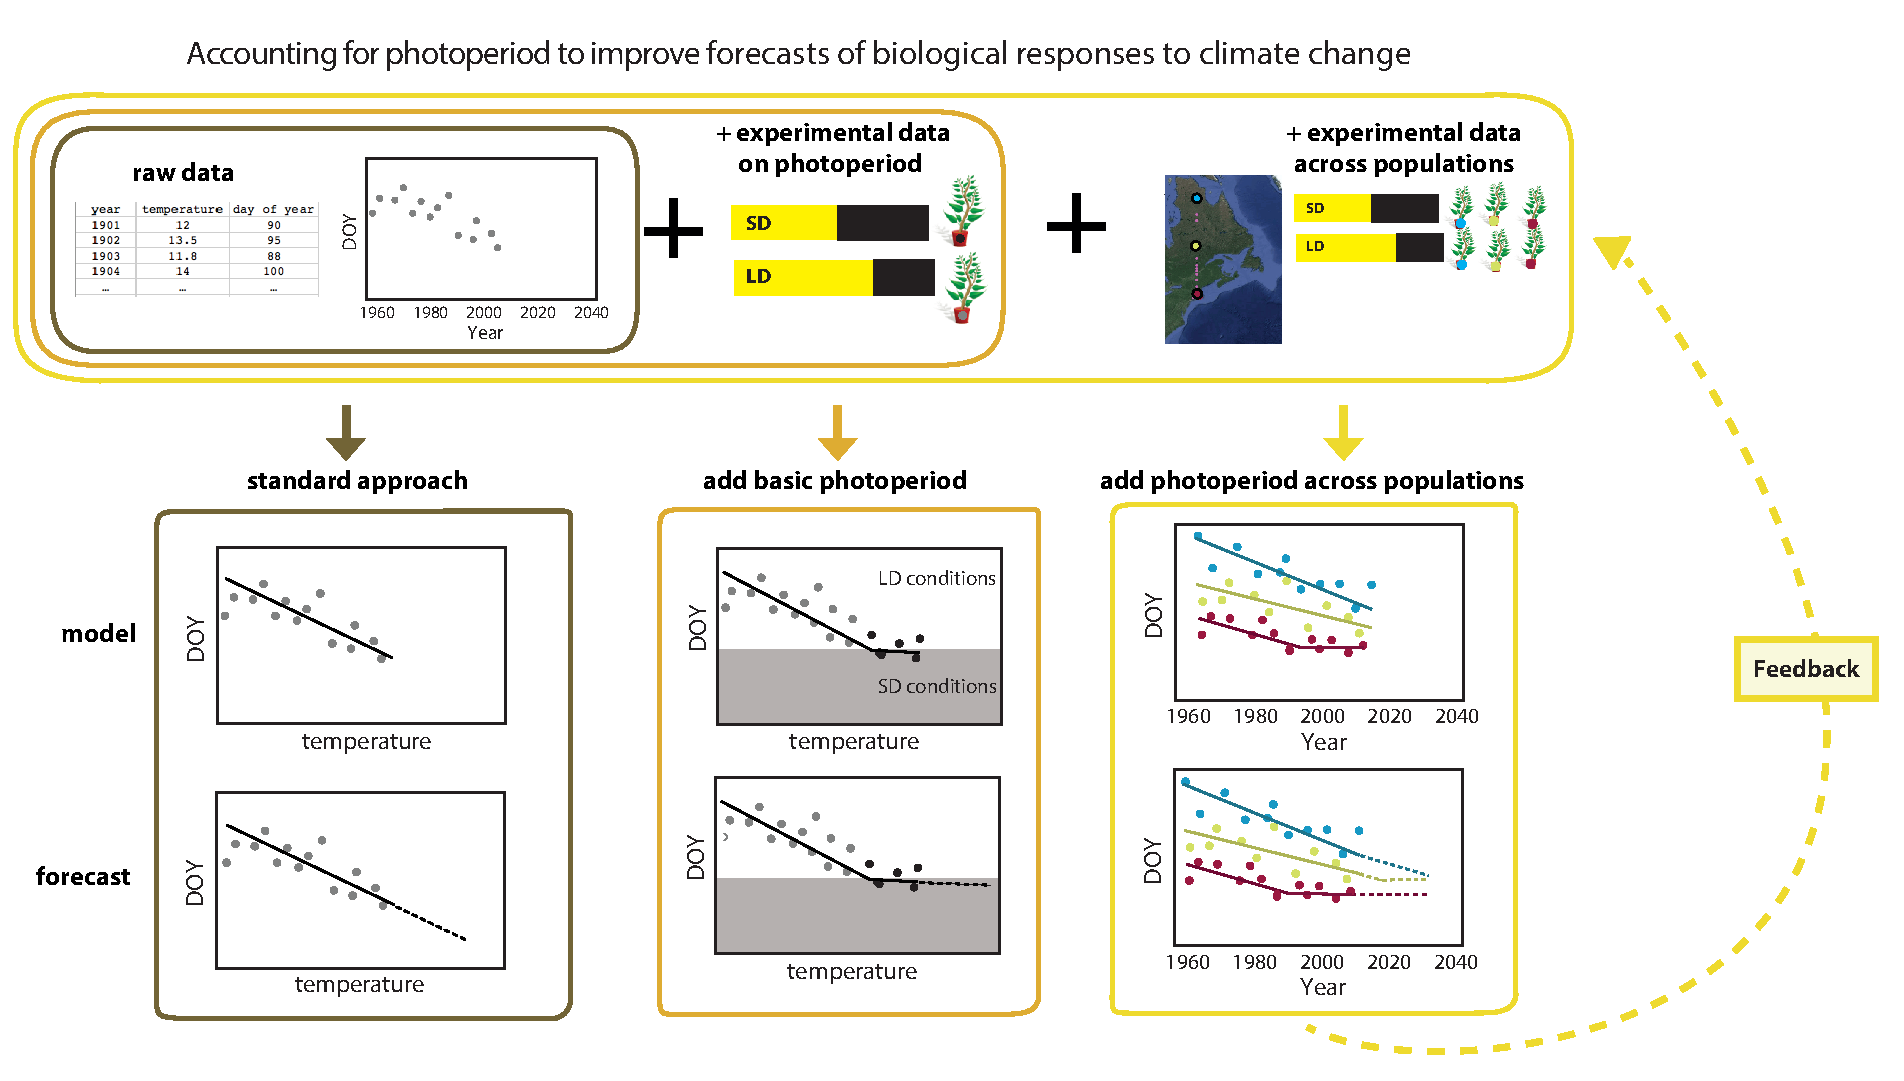
\includegraphics{..//..//analyses/photoperiod/figures/photocondiag6.pdf} 
\caption{\textbf{Conceptual diagram of how to include photoperiod in forecasting biological responses to climate change}. Current approaches for forecasting spring phenology with climate change frequently rely on linear relationships between historical temperature data and observed dates of spring phenology (left panels). Adding responses to photoperiod, which may operate as threshold responses to short days (SD) versus long days (LD, see `photoperiod sensitivity' in Table 1 and Box 2 for details), will alter these forecasts (center panel) in ways that differ across species with divergent threshold photoperiods. Other factors that interact with photoperiod, such as population-level variation in photoperiod responses, can be incorporated into forecasts to further improve their accuracy (right panel).}
 \label{fig:condiag}
 \end{figure}
\clearpage

 
 \section*{Box 1. Are photoperiod effects widespread? A case study of woody plant spring phenology}
\par Photoperiod responses are well-studied in woody plant phenology, making this a useful case study to consider climate change-induced shifts in photoperiod. Spring woody plant phenology in particular has critical implications for global carbon cycling and feedbacks to the climate system \citep{richardson2013}, and has been at the center of an important and controversial debate on the relative effects of photoperiod versus temperature on phenology \citep[e.g.,][]{fu2019,chuine2010,koerner2010a,koerner2010b}. 

\par Experimental growth chamber studies have shown that photoperiod is an important cue for spring budburst phenology in woody plants \citep[e.g.,][]{flynn2018,Basler:2014aa,Heide:1993a}. These experiments often manipulate photoperiod in combination with temperature to address basic questions about how these two environmental conditions act as biological cues. Temperature has a dual role in regulating woody plant phenology: chilling---the prolonged exposure to cold temperatures after growth cessation in the fall---is required to initiate budburst, and forcing---prolonged exposure to warm temperatures---is required for budburst to occur. Different photoperiod treatments are typically applied during the forcing treatment phase in growth chamber experiments \citep[e.g.,][]{Laube:2014a,Spann:2004aa,Falusi:1990aa,HEIDE:1977aa,Campbell:1975aa}. 

\par Woody plant growth chamber studies have been conducted for decades, but have only recently been synthesized to show that photoperiod sensitivity is widespread, with large variation across studies and species. These studies were aggregated in Observed Spring Phenology Responses in Experimental Environments (OSPREE), a new database of plant growth chamber studies that manipulate photoperiod and temperature to measure plant phenological responses, such as budburst and flowering \citep{wolkovich2019}. The database includes studies that manipulate photoperiod (by applying treatments with different daylength durations, applying long-day versus short-day conditions for different lengths of time, and/or applying varying versus constant photoperiods) and temperature (by imposing different chilling and/or forcing treatments). The OSPREE database spans 201 woody plant species; all experiments in the database use dormant plant tissue (grown in greenhouses or taken directly from the field) exposed to experimental conditions for which we could identify forcing, photoperiod, and chilling treatments quantitatively. See Methods S1 of the \emph{Supporting Information}, \citet{ettinger2020}, and \citet{wolkovich2019} for details. 


\par Growth chamber experiments in OSPREE suggest that the dominant photoperiod response in woody plant species is earlier and more rapid budburst with longer days \citep [e.g., ][]{Caffarra:2011a}. Thirty of the 72 studies in the OSPREE database included two or more different photoperiod treatments. Of these, 26 (87\%) found significant photoperiod main effects or significant interactive effects with temperature (i.e., photoperiod x temperature effects), across 176 species (Table S1). Main effects included responses such as growth \citep[e.g., higher growth rates with longer days][]{Ashby:1962aa} and reproduction \citep[e.g., increased flowering with longer days][]{Heide:2012aa}. 


\par Growth chamber experiments highlight that responses to photoperiod vary depending on temperature conditions. For example, an accelerated advance of budburst was observed under long versus short days with low chilling, relative to bubdburst with high chilling in \emph{Betula payrifera} \citep[][see Fig. Box 1-1]{Hawkins:2012}. Similarly, across species, as chilling accumulates from winter to spring, sensitivity to both forcing and photoperiod sensitivity can decrease \citep{malyshev2018}. Frequently, long photoperiods can compensate for low amounts of chilling \citep{Caffarra:2011b,Myking:1995,Heide:1993}.%or low forcing?
\par Woody plant growth chamber experiments also demonstrate that, though photoperiod responses are common, they are variable, as shown in Fig. Box 1-1. Responses to photoperiod differ by species \citep[e.g.,][]{flynn2018,zohner2016,Basler:2014aa,Basler:2012,Howe:1996,Heide:1993a}.
For example, with longer chilling treatments some species seem insensitive to daylength \citep[e.g., \emph{Hammamelis} spp., \emph{Prunus} spp.,][]{zohner2016}, whereas others seem to be highly sensitive to daylength (e.g. \emph{Fagus} spp., Fig. \ref{fig:fagus}A), even with long chilling treatments \citep{zohner2016}. In addition, some species demonstrate a response to photoperiod opposite to that typically observed: \emph{Tilia}, for example, showed delayed budburst with longer daylengths \citep[see Fig. Box 1-1,][]{Ashby:1962aa}.
Photoperiod sensitivity also varies by population and ecotype (e.g., Fig. Box 1-1). For example, photoperiod effects on budburst were more significant for lower latitude populations of \emph{Betula pendula} and \emph{B. pubescens} \citep{Partanen:2005aa}. 

\makeatletter
\renewcommand{\thefigure}{Box 1-\@arabic\c@figure}
\makeatother
\setcounter{figure}{0}
\begin{figure}[h]
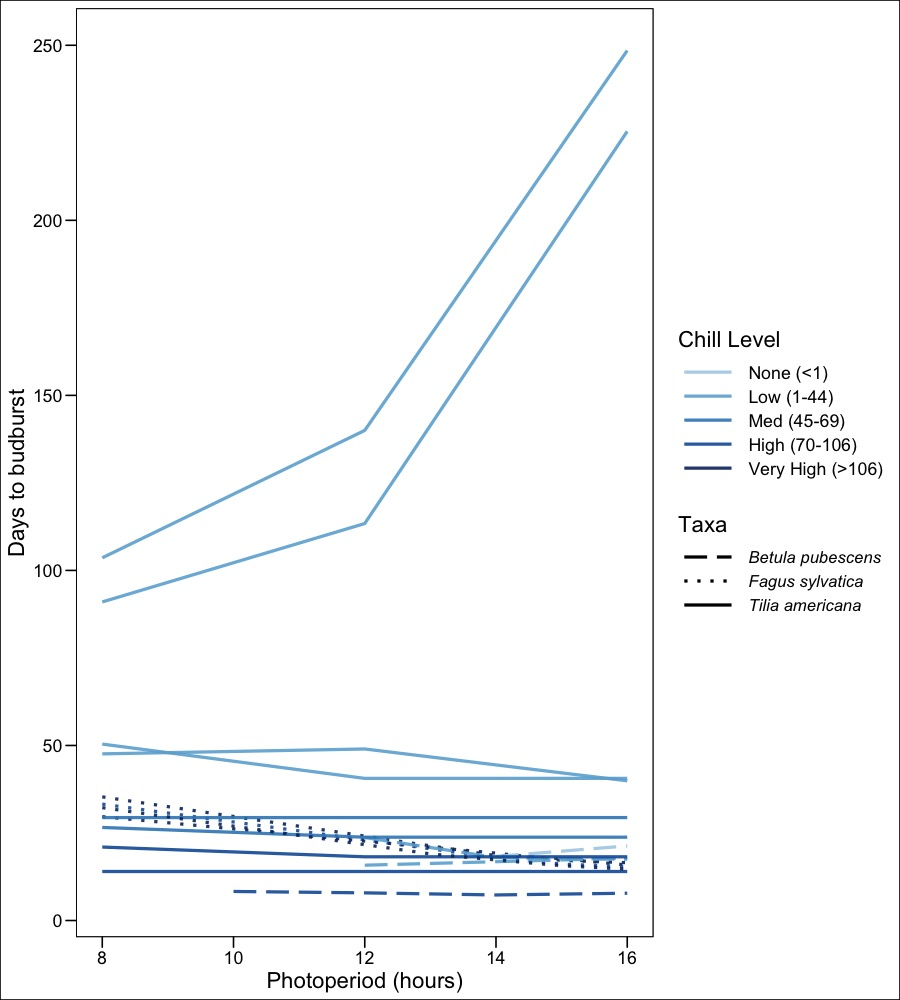
\includegraphics{..//..//analyses/photoperiod/figures/Photo_curv_version2blue.jpeg} 
\caption{\textbf{ Nonlinearities in phenological responses to daylength} are apparent in spring woody plant phenology experiments. Shown are responses from all experiments  from \citet{wolkovich2019}in which three or more photoperiod treatment levels were applied. The shape of the response curves for \textit{Betula pubescens} \citep{Caffarra:2011b}, \textit{Fagus sylvatica} \citep{Heide:1993a} and \textit{Tilia americana} \citep{Ashby:1962aa} differ depending on the amount of winter chilling received \citep[measured in Chill portions,][with darker blue indicating more chilling]{fishman1987}. Species and chilling levels with multiple lines represent plant material from different populations. See ``Nonlinearities in phenological responses to daylength'' in Methods S1 of the \emph{Supporting Information} for additional details.}

\label{fig:photocurve}
\end{figure}

\begin{figure}[h]
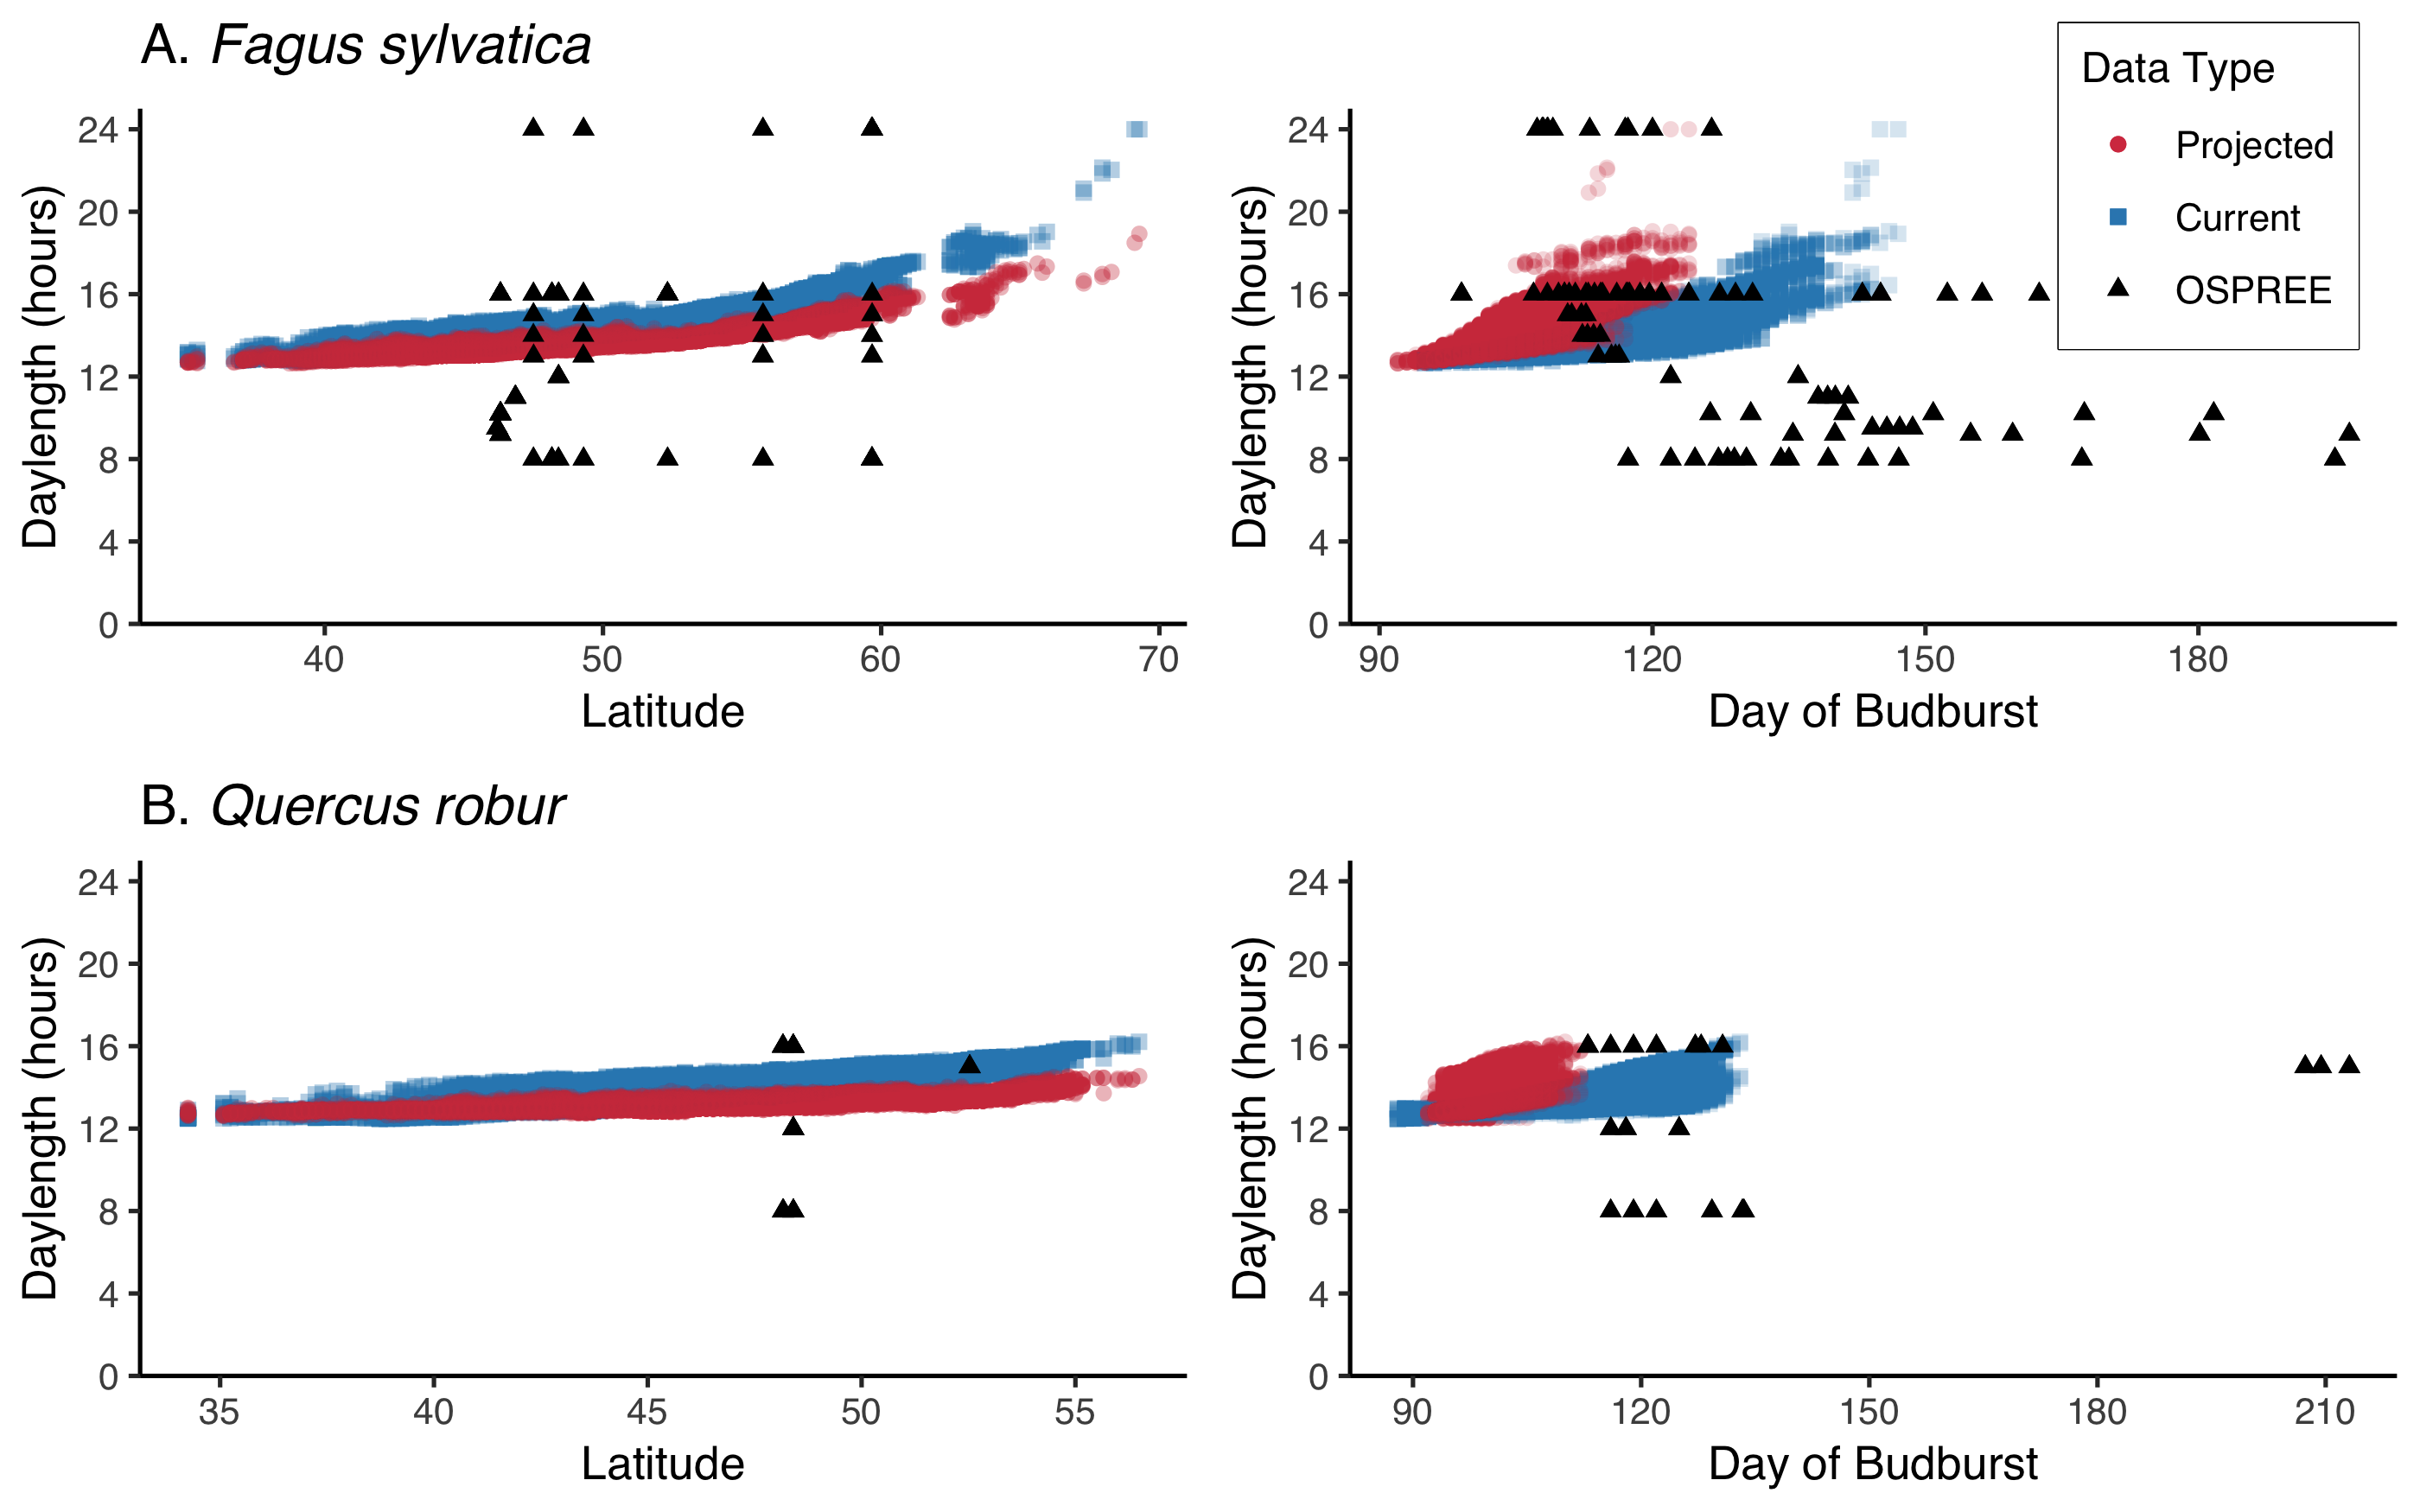
\includegraphics{..//..//analyses/photoperiod/figures/2D_actual_combined.png} 
\caption{\textbf{Experienced photoperiods in growth chamber experiments differ from those in the natural world}, shown here by latitude (left panels) and by day of budburst (right panels) for \emph{Fagus sylvatica} (A, upper panels) and \emph{Quercus robur} (B, lower panels). Triangles show experimental treatments of photoperiod in \citet{wolkovich2019}. To illuminate potential gaps between experiments and the natural world, we show the photoperiod when budburst occurs in its current (1981-2000) and projected ranges \citep[2081-2100, using the A1Fi Phenofit scenario, see][]{duputie2015}. We scaled the days to budburst for all data points in \citet{wolkovich2019} by adding the day of budburst from the first Phenofit observation. See ``Comparing shifts in experienced photoperiod in experiments to those in the natural world with climate change'' in Methods S1 of the \emph{Supporting Information} and \citet{duputie2015} for additional details.} 
 \label{fig:fagus}
 \end{figure}
 
\clearpage 
\section*{Box 2. Dominant models of how photoperiod affects spring woody plant phenology}
\par The cues and molecular pathways underlying photoperiod sensitivity are poorly understood for most organisms, even in relatively well-studied phenophases and taxa, such as spring budburst in woody plants \citep{ding2016}. Decades of growth chamber experiments demonstrate that three main cues---chilling, forcing, and photoperiod---control spring budburst for woody species \citep{flynn2018, zohner2016,Heide:2008aa}, with many models suggesting a dominant role of forcing in most natural conditions. Forcing requirements, however, appear to increase given shorter photoperiods or lower chilling \citep{Caffarra:2011qf,chuine2010}. Research has yet to fully tease out effects of these three cues, their interactions, and their prevalence;  photoperiod responses appear variable across species and populations, as well as with different chilling treatments (see Box 1). Not surprisingly, there is currently little agreement on the underlying model for how photoperiod affects spring phenology for most species \citep{chuine2016,hanninen2019}. More physiological research will likely be necessary for major advances, as understanding the exact cellular pathways through which chilling, forcing, and photoperiod act appears increasingly critical to accurate modelling \citep{vanderschoot2014,hanninen2019}. 

\par Additional cellular and molecular studies may quickly advance understanding and scale up to improved photoperiod models. While our understanding of how plants interpret photoperiod at the molecular-level comes from few species, largely from studies of flowering in the model plant \emph{Arabidopsis thaliana} \citep[e.g.,][]{suarez2001} and fall budset in woody plant species \citep[e.g.,][]{Howe:1996}, these studies have proved useful across other species. For example, the `external coincidence model' \citep[where plants sense light via blue light receptors and phytochromes, then interpret photoperiod through a coordinated response to light in relation to the time of day, see][]{lagercrantz2009} has been most widely studied in \emph{Arabidopsis}, but appears to be a relevant mechanism for photoperiod responses in diverse perennial and woody plant species \citep{Singh:2017,petterle2013,andres2012,kobayashi2007,davis2002,bastow2002,bunning1936}. The model proposes the existence of a circadian rhythm of light sensitivity, in which the night-phase is sensitive to light and the day-phase is insensitive to light. As days get longer in the spring, daylight illuminates the light sensitive phase, triggering a response. This provides a clear mechanistic pathway to build into models \citep{Burghardt2015}. 

\par We expect progress on spring phenology will benefit from similar physiological research that spans the molecular to whole-plant levels. To date, little is known about the genetic pathways responsible for the light-sensing apparatuses involved in spring budburst, and how they may vary across species or populations. Some genes have been identified that play a role in coordinating budburst in poplar (\emph{Populus} spp.), and may occur in other woody species as well. Many similarities exist between the proposed regulatory networks of vegetative growth in \emph{Populus} and those controlling floral initiation in \emph{Arabidopsis}, \citep{ding2016}. For example, vegetative growth and inhibition of budset are promoted by the FLOWERING LOCUS T2 (FT2) gene, a homolog of \emph{Arabidopsis thaliana} gene FLOWERING LOCUS (FT). FT2 expression appears to be controlled by a pathway that is effective in long days and warm temperatures, marking the onset of the growing season \citep{Hsu:2011}. Its loss of expression in autumn, when the days are getting shorter, is associated with the onset of dormancy \citep{glover2014}.

\par Efforts to better map the genetic and cellular pathways of spring phenology combined with common garden studies can provide a powerful method to test mechanistic understanding and improve models \citep[e.g.,][]{Burghardt2015,fournier2016}. Here we have mainly outlined how to combine growth chamber studies with long-term data to improve models and forecasting; a greater physiological understanding of at least a few species will likely also be necessary for generating robust predictions with climate change.

%%%%%%%%%%%%%%%%%%%%%%%%%%%%%%%%%%%%%%%%
\end{document}
%%%%%%%%%%%%%%%%%%%%%%%%%%%%%%%%%%%%%%%%
